% \pagebreak[4]
% \hspace*{1cm}
% \pagebreak[4]
% \hspace*{1cm}
% \pagebreak[4]


\ifpdf
    \graphicspath{{pic/}}
\else
    \graphicspath{{pic/}}
\fi

\chapter{ Virtual Observatory (VO)}

% \begin{lstlisting}[frame=single]
% What is the motivation behind Virtual Observatory? Is data avalanche
% problem only in astronomy? What is IVOA?  What is Virtual Observatory
% architecture?
% \end{lstlisting}

\begin{figure}[!htbp]
  \begin{center}
    \leavevmode
    \ifpdf
    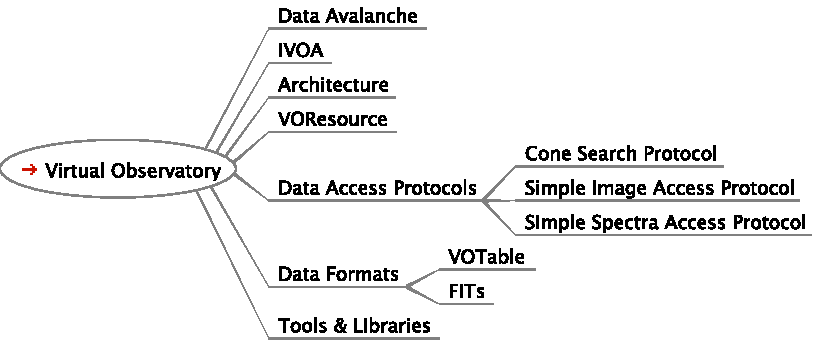
\includegraphics[scale = 1]{mapVirtualObservatory}
    \else
    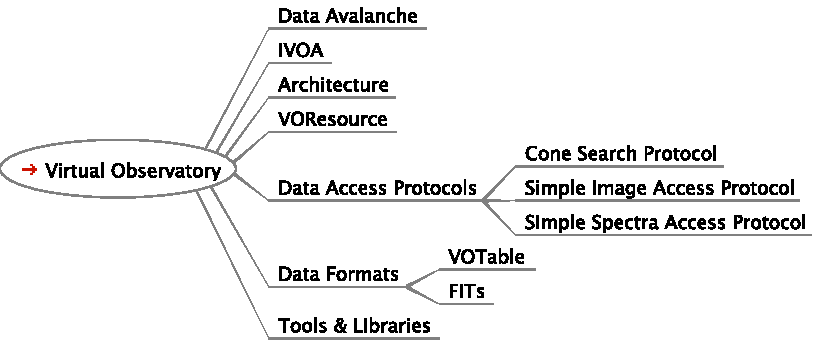
\includegraphics[bb = 92 86 545 742, height=6in]{mapVirtualObservatory}
    \fi
    \caption{Chapter structure}
    \label{FigStructure}
  \end{center}
\end{figure}

\section{ Data avalanche: Opportunity or disaster?}

There are two important trends in current astronomy surveys:

\begin{itemize}

  \item{Size:} The cumulative compressed data holdings of the ESO archive will
    reach 1 PetaByte by 2012 \cite{hanisch2010international}. Projects
    like Large Synoptic Survey Telescope (LSST) will produce about 30
    TB per night, leading to a total database over the ten years of
    operations of 60 PB for the raw data \cite{becla2006designing}.
   
  \item{Complexity:} Modern surveys will cover the sky in different
    wave-bands, from gamma- and X-rays, optical, infrared to
    radio. The ability to cross correlate these observations together
    may lead to new understanding of physical
    phenomenas. \cite{hanisch2010international}
\end{itemize}



Such an amount of data is not possible to transfer over the
network. Data resources are heterogeneous, distributed and
decentralized in nature.


There is an interesting analogy with the problem (and the solution)
which scientists discovered during LEP project at CERN.  Their problem
was too many documents in different formats. Tim Berners-Lee\footnote{
  Sir Timothy John "Tim" Berners-Lee. British engineer and computer
  scientist and MIT professor credited with inventing the World Wide
  Web.} designed set of protocols (URIs, HTTP and HTML) which allowed
link and share documents\cite{berners1990worldwideweb}. This was
recognized as generally useful and World Wide Web was born. An
important role plays the World Wide Web Consortium (W3C) in developing
Web standards\footnote{Prior to its creation, incompatible versions of
  HTML were offered by different vendors, increasing the potential for
  inconsistency between web pages.}.
    
    
\section{International Virtual Observatory Alliance (IVOA)}

   \begin{wrapfigure}{r}{0.7\textwidth}
     \vspace{0pt}
     \begin{center}
       \ifpdf
       
\includegraphics[width=0.7\textwidth]{ivoamembers}
       \else
       
\includegraphics[bb = 92 86 545 742, height=6in]{ivoamembers.jpg}
       \fi
     \end{center}
     \vspace{-20pt}
     \caption{IVOA members}
     \vspace{-10pt}
   \end{wrapfigure}


   What is necessary is sets of standards and protocols to deal with
   heterogeneous distributed data and authority which encourages their
   implementation. Such an authority is the International Virtual
   Observatory Alliance (IVOA). It comprises 19~VO programs from
   Argentina, Armenia, Australia, Brazil, Canada, China, Europe,
   France, Germany, Hungary, India, Italy, Japan, Russia, Spain, the
   United Kingdom, and the United States and inter-governmental
   organizations (ESA and ESO)\cite{hanisch2010international}.
   
    Standards and specifications produced by IVOA can be obtained at
    \url{http://www.ivoa.net/}.

    %% \begin{figure}[!htbp]
    %%   \begin{center}
    %%     \leavevmode
    %%     \ifpdf
    %%     
\includegraphics[height=6cm]{ivoamembers}
    %%     \else
    %%     
\includegraphics[bb = 92 86 545 742, height=6in]{ivoamembers}
    %%     \fi
    %%     \caption{IVOA members}
    %%     \label{FigAir}
    %%   \end{center}
    %% \end{figure}


\section{Architecture}
    % The Virtual Observatory is the  “middle layer” framework
    % which connects the Resource Layer to the User Layer in a seamless
    % and transparent manner. The objective is to improve and unify access to
    % astronomical data and services.

 
The Architecture is depicted on the figure \ref{FigArchitecture}. The
level of abstraction goes from top to bottom. Starting with interfaces,
used by people or applications to discover resources.  Next level is
the service layer implemented by standard protocols, followed by the
hardware level where actual data are stored. This onion like structure
hides the complexity of the lower layer and provide data and meta-data
to the higher layer. This concept is similar to TCP/IP
\footnote{TCP/IP (Transmission Control Protocol/Internet Protocol).
  The basic communication language or protocol of the Internet.}
protocol.


 
    \begin{figure}[!htbp]
      \begin{center}
        \leavevmode
        \ifpdf
        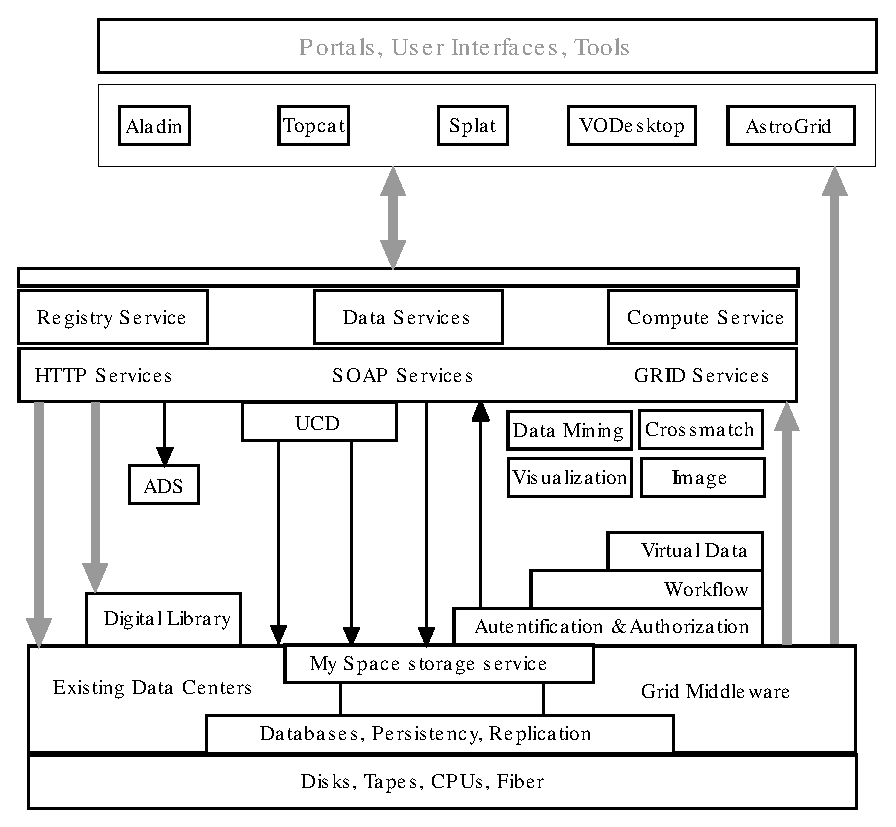
\includegraphics[scale = 1]{architecture}
        \else
        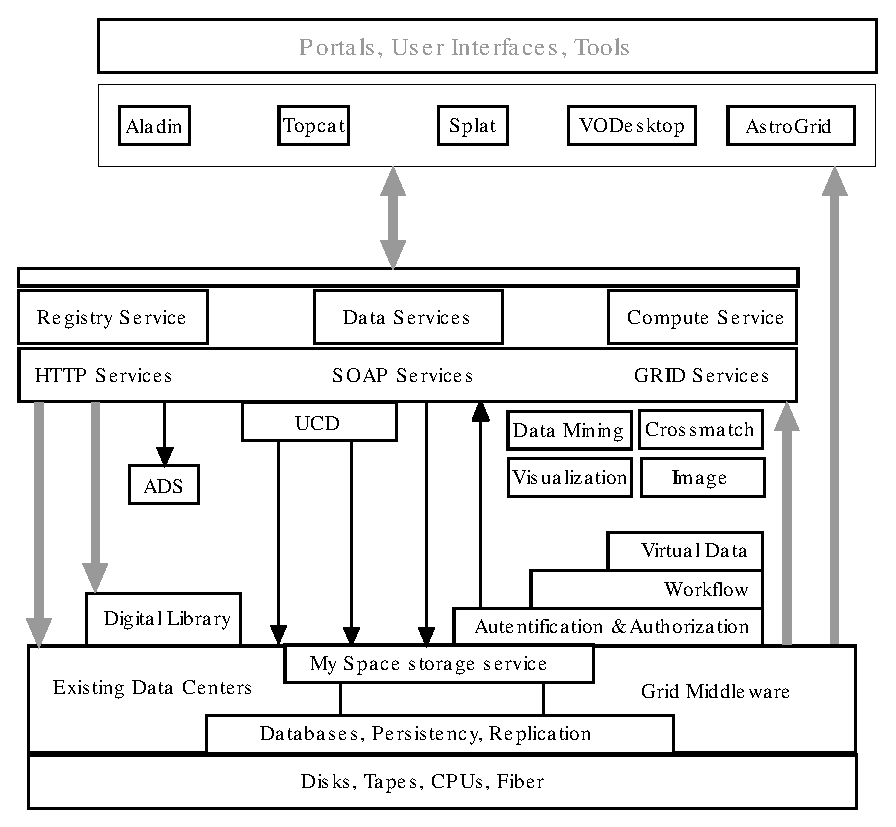
\includegraphics[bb = 92 86 545 742, height=6in]{architecture}
        \fi
        \caption{VO Architecture}
        \label{FigArchitecture}
      \end{center}
    \end{figure}

\clearpage

The VO architecture is serviced oriented. Each service is autonomous
with well defined defined boundaries. Very important aspect of VO
implementation is the adoption of formats and protocols used in
astronomy (FITS) and Computer Science (XML \footnote{Extensible
  Markup Language (XML) is a set of rules for encoding documents in
  machine-readable form.} , Web service \footnote{method of
  communication between two electronic devices over a network.} SOAP
\footnote{Simple Object Access Protocol, is a protocol specification
  for exchanging structured information in the implementation of Web
  Services in computer networks.}) for many years. In other words VO
does not try to reinvent the wheel but it stands on the shoulders of
giants.


\section{VOResources}

A resource is a general term referring to a VO element that can be
described in terms of who curates or maintains it and which can be
given a name and a unique identifier. Just about anything can be a
resource: it can be an abstract idea, such as sky coverage or an
instrumental setup, or it can be fairly concrete, like an organization
or a data collection. \cite{bensonivoa}

UML\footnote{Unified Modeling Language. Standardized general-purpose
  modeling language in the field of object-oriented software
  engineering.}  diagram of the resource is on the figure
\ref{FigResource}. Next paragraph is an attempt to explain this
diagram to non-programmers. Full arrow means generalization, Resource
can be a generalization of organization, data collection, application
or service. Single arrow means association. Organization can be linked
(associated) together with other organization (multiplicity is
represented by number 1, 0..). The same is true for data
collection. Organization is a generalization of and/or provider which
can own zero to N services. Diamond means the aggregation. Publisher
can have any resources.
  
    \begin{figure}[!htbp]
      \begin{center}
        \leavevmode
        \ifpdf
        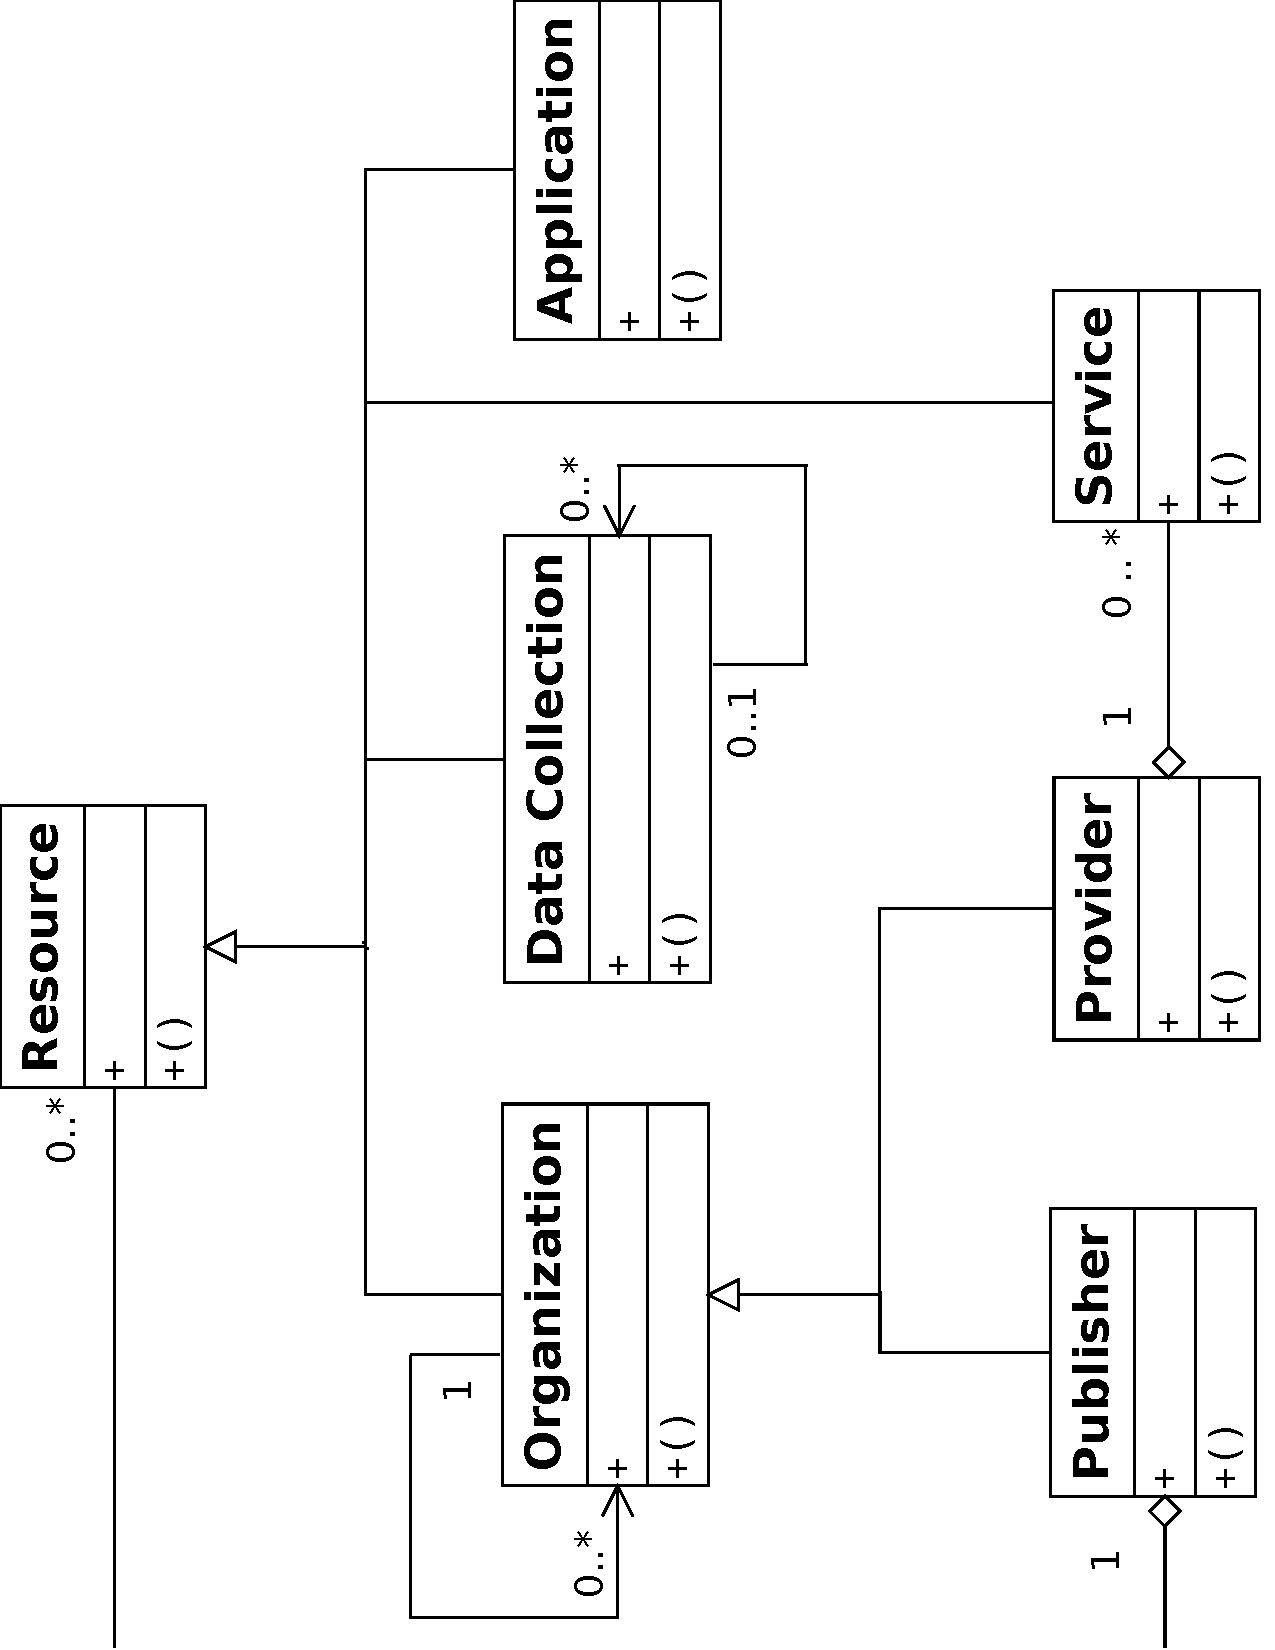
\includegraphics[scale = 1]{resources}
        \else
        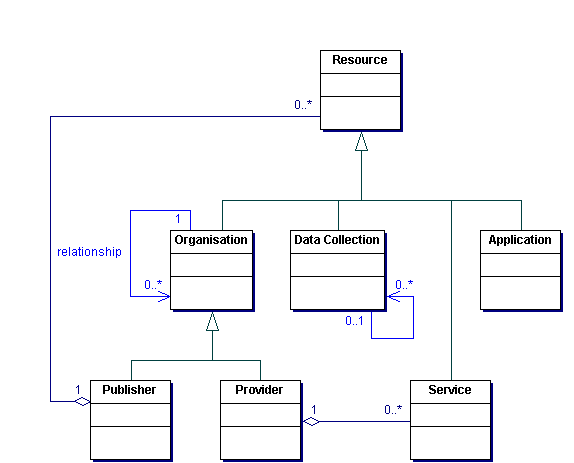
\includegraphics[bb = 92 86 545 742, height=6in]{resource.png}
        \fi
        \caption{UML diagram of VOResource}
        \label{FigResource}
      \end{center}
    \end{figure}

\clearpage

Following example uses program stilts\footnote{STIL Tool Set. Set of
  command-line tools based on STIL, the Starlink Tables Infrastructure
  Library.} to query registry with parameter shortName equal to
'AIASCR'\footnote{Astronomical Institute of the Academy of Sciences of
  the Czech Republic}. This returns VOTable containing meta-data
about the resource. 

\begin{lstlisting}[frame=single]
stilts regquery query="shortName like 'AIASCR'"
regurl=http://registry.euro-vo.org/services/RegistrySearch
ofmt=votable-tabledata > resourceExample.vot
\end{lstlisting}

Rows 1--4 define XML nad VOTable schema with adequate locations
(xmlns\footnote{XML namespaces. Provide uniquely named elements and
  attributes in an XML document.}) followed by informations about the
actual resource. The listing is abbreviated.

  \input{resourceExample.vot}

    
% \section{VOregistry}
%     Is the standard defined by IVOA for registration of VO-Resources

%     The IVOA Registry enables users and applications in the User Layer
%     to discover data and metadata collections, as well services in the
%     Resource Layer.  A resource is a general term referring to a VO
%     element that can be described in terms of who curates or maintains
%     it and which can be given a name and a unique Resource Identifier.
%     A resource can be of various types: a data or metadata collection,
%     a computing or storage element, an application, a data and
%     metadata access service, etc. \cite{gray2007}
    

%     \begin{figure}[!htbp]
%       \begin{center}
%         \leavevmode
%         \ifpdf
%         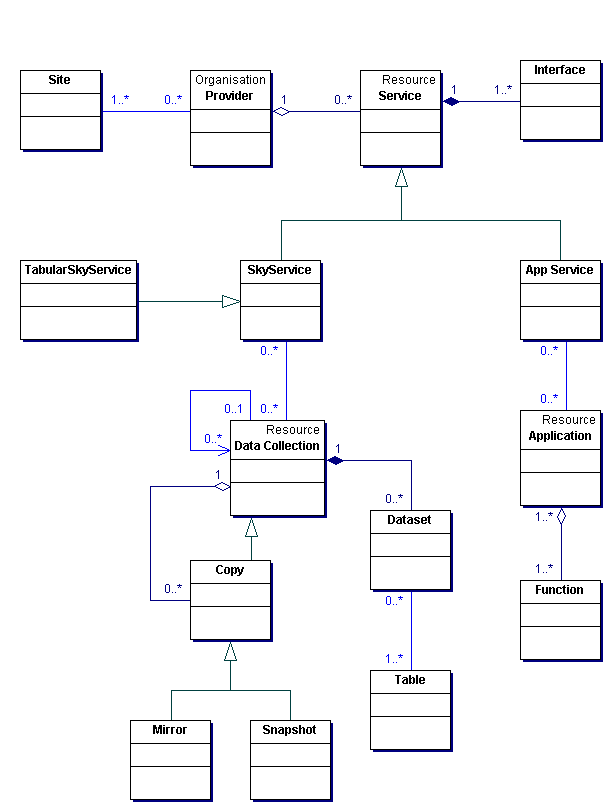
\includegraphics[height=15cm]{registry}
%         \else
%         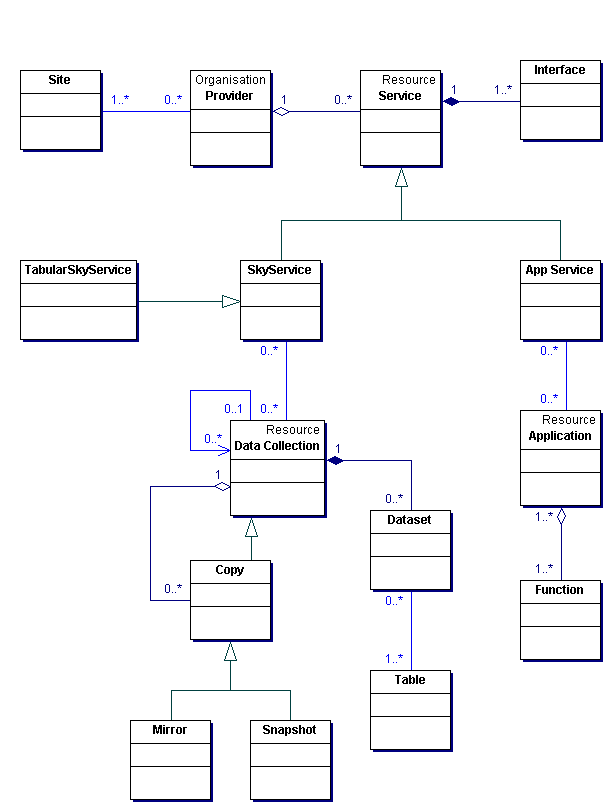
\includegraphics[bb = 92 86 545 742, height=6in]{registry}
%         \fi
%         \caption{UML diagram of VORegistry}
%         \label{FigRegistry}
%       \end{center}
%     \end{figure}


% autonomous, and its boundaries well-defined
% inherently distributed

% picture from
% http://www.ivoa.net/cgi-bin/twiki/bin/view/IVOA/RegistryUseCases

% \clearpage

\section{Data Access Protocols}

Protocols are very important part of Virtual Observatory. Their
understanding is key to comprehend the concepts behind VO. They allow
to discover resource and obtain desirable data. All of them are based
on existing web standards and are designed to be simple and therefor
easy to implement on existing astronomical archives. The main idea is
simple and universal: HTTP GET request with parameter is sent to the
resource and structured document (VOTable) is sent back.

\subsection{Cone Search Protocol} \label{sec:csp}
Cone Search was the first standard protocol of Virtual Observatory. It
enables to retrieve records from an astronomical catalog. The input is
the query which describes sky position and the radius on the sky. The
output is a list of objects whose positions lie in the defined
vicinity. The output is formatted as a VOTable. Service compliant with
Cone Search Protocol is called Cone Search Service. Only the request
and response is specified not the implementation or data storage.


The requirements are:


\begin{enumerate}
\item Respond to a HTTP GET request represented by a URL 

\begin{lstlisting}
  http://<server-address>/<path>?[<extra-GET-arg>&[...]]
\end{lstlisting}

The constrains are expressed as a list of ampersand-delimited GET
arguments. For example:

\begin{lstlisting}
  http://simbad.u-strasbg.fr/simbad-conesearch.pl?RA=24.5&DEC=-57.2&SR=0.1
\end{lstlisting}

Where RA is right-ascension, DEC declination and SR the radius of the
cone in the ICRS coordinate system in decimal degrees. These
parametrers are requied others are optional.

\item Return an XML document in the VOTable format.  

  There are several requirements on the contents of the table:

  \begin{itemize}
  \item UCD fields "ID\_MAIN", "POS\_EQ\_RA\_MAIN", "POS\_EQ\_DEC\_MAIN" must
    be present.
  \item Return VOTable with single PARAM element name="Error" in the
    case of error.
  \end{itemize}

\end{enumerate}

Cone Search is implemented in many software packages. Besides standard
VO tools like TOPCAT or STILTS also in MUNIPACK and many others.
Following example shows simple query to SIMBAD \cite{wenger2000simbad}
catalog using method \emph{urlopen} of Python library \emph{urllib2}.
 
\begin{lstlisting}
  import urllib2
  response = urllib2.urlopen('http://simbad.u-strasbg.fr/simbad-conesearch.pl?RA=24.5&DEC=-57&SR=0.1')
  print response.read()
\end{lstlisting}

\noindent The same result can be obtained using program like wget\footnote{program
  for non-interactive download of files from the Web} or Web browser.

\subsection{Simple Image Access Protocol}
The key idea behind the SIA Protocol is to allow users and programs to
retrieve images created by an image service on-the-fly. From technical
point of view it is designed in a similar way as Cone Search Protocol
(see \ref{sec:csp}), specifically as name-value HTTP GET requests and
the VOTable XML format output. The user specifies ideal image coverage
(position and the size) he wants to receive and the image service
produces a list of images it can return in the VOTable format. The
user then could issue getImage request to retrieve desirable images.

There are following requirements for compliance. To be a SIA service
To be a SIA service, it must support:

\begin{itemize}
\item Image Query web method,
\item Image Retrieval (getImage) web method.
\end{itemize}

\noindent Furthermore the image service should be registered to be
able to locate optimal service. There are several types of image
services:

\begin{itemize}
\item Image Cutout Service.

  Provides rectangular regions of large images.
\item Image Mosaicing Service.

  Size, scale and projection could be specified.
\item Atlas Image Archive

  Pre-computed atlas of images.
\item Pointed Image Archive.  

  Images are not part of a sky survey but
  rather focused on specific source
\end{itemize}


To get a list of images query has to send via HTTP GET method. The
first part is base URL. The second part are parameters specifying image
properties such as position (POS), size (SIZE), etc.

\begin{lstlisting}
  http://<server-address>/<path>?[<extra GET arg>&[...]]
\end{lstlisting}

There are two examples of using SIA protocol to obtain image. First
one from SDSS, second from Hubble Space Telecope archive. 

\begin{lstlisting}
  http://skyview.gsfc.nasa.gov/cgi-bin/vo/sia.pl?SURVEY=SDSS&POS=18.87667,-0.86083&SIZE=1
  http://hubblesite.org/cgi-bin/sia/hst_pr_sia.pl?POS=83.6,22.0&SIZE=1.0
\end{lstlisting}

There is more complex example using Astrogrid framework to show how to
discover SIA service and obtain an image. First registry method
searchSiap is used to find SIA service for SDSS, this is then used in
SiapSearch method to obtain result in VOTable format.  

\begin{lstlisting}
  In [1]: from astrogrid import Registry, ConeSearch
  In [2]: list = reg.searchSiap('SDSS')
  In [3]: print [p['id'] for p in list]
  -------> print([p['id'] for p in list])
  ['ivo://nasa.heasarc/skyview/sdss']
  
  In [4]: siap = SiapSearch('ivo://nasa.heasarc/skyview/sdss')
  In [5]: result = siap.execute(18.8, -0.8, 1.0)
\end{lstlisting}

% Even more sophisticated example is described below. The STILTS tool is
% used to get images from 2MASS survey for many objects from the file
% using SIA protocol. This file is the list of Be starts from Ondrejov
% used later in this work.


 

\subsection{Simple Spectra Access Protocol}

SSA Protocol allows to discover and obtain 1-D spectra from VO
Service. It shares many similarities to the previously discussed SIA
Protocol.

defines a uniform interface to remotely discover and access simple 1-D spectra. 

similar to that of the older Simple Image Access (SIA)

The process to obtain a spectrum compose of following steps:

\begin{itemize}
\item Query the resource registry.
\item Data discovery to selected service to get aviable resources in
  VOTable format.
\item Download selected spectra using URL.
\end{itemize}

The spectra could be one of the following types:

\begin{itemize}
\item Pre-computed
\item Computed on the fly
\end{itemize}

To be a SSA-compliant, the service must provide:

\begin{enumerate}
\item HTTP GET interface, returning the query response encoded as a
VOTable document, with at least parameters POS, SIZE, TIME, BAND, and FORMAT.
\item GetData method returning data in at least one of the
  SSA-compliant data formats (VOTable, FITS)
\item FORMAT=METADATA� metadata query feature
\end{enumerate}


Following example show how to discover resources with SSA capability
using STILTS program. 

\begin{lstlisting}
  stilts regquery query="shortName like 'ESO' capability/@standardID =
  'ivo://ivoa.net/std/SSA'" ocmd="keepcols 'ShortName accessUrl'"
  ofmt=ascii
\end{lstlisting}

With information of service URL, one can specify a query to obtain a
list with aviable spectra in VOTable format. This can be used in Web
browser or via programs such \emph{wget} or \emph{curl}.

\begin{lstlisting}
  http://archive.eso.org/apps/ssaserver/EsoProxySsap?REQUEST=queryData&POS=83.63,22&SIZE=1
\end{lstlisting}

\section{Data Formats}
Astronomy has always been, by its nature, on vanguard of image
producing and processing. This is especially true for the era of
digitalization. The situation with data formats in astronomy is
unique. There are just few very good standards with variety of
implementation in many programming languages. Virtual Observatory
takes advantage of this heritage and implement these formats in
sensible way into its own standards. 
 
\subsection{VOTable}
\subsubsection*{Motivation}
VOTable is flexible storage and exchange format fundamentally
interconnected with Virtual Observatory. It has features for big-data
and Grid computing. Data can be stored in different ways in dependence
on the charatecter and size. Small tables can be stored in pure XML
\footnote{Extensible Markup Language. W3C standard. Set of rules for
  encoding documents in machine-readable form}, while large-scale data
can be referenced with the URL \footnote{Uniform Resource
  Locator. Uniform Resource Identifier (URI) that specifies where an
  identified resource is available and the mechanism for retrieving
  it.} syntax protocol://location.  It combines web standards (it is
based on XML) and astronomy tradition in storing data (it is FITS
compatible). Expiration and authentication are also supported.

\subsubsection*{Structure}
Following example of VOTable was created from SDSS FITS file used in
this work. First there is an information about XML and VOTable
versions and references to corresponding XML Schema \footnote{Define
  the legal building blocks of an XML document. Note: XML schema can
  be described by XML Schema, Document Type Definition (DTD) or RELAX
  NG }. <TABLE> tag encapsulating tabular data. <FIELD>
tag describe identifinaction (ID), type and precision of
columns. <DATA> tag contains data (here) in TABLEDATA format (other
types are FITS and BINARY)
 
\begin{lstlisting}
<?xml version="1.0" encoding="utf-8"?>
<!-- Produced with vo.table version 0.6
     http://www.stsci.edu/trac/ssb/astrolib
     Author: Michael Droettboom <support@stsci.edu> -->
<VOTABLE version="1.0"
 xmlns:xsi="http://www.w3.org/2001/XMLSchema-instance"
 xsi:noNamespaceSchemaLocation="http://www.ivoa.net/xml/VOTable/v1.0"
 xmlns="http://www.ivoa.net/xml/VOTable/v1.0">
 <RESOURCE type="results" >
  <TABLE >
   <FIELD ID="col0" name="wave" datatype="float" unit=""
   precision="F9"/>
  <DATA>
    <TABLEDATA>
     <TR>
      <TD>4012.50757</TD>
     </TR>
 </TABLEDATA>
   </DATA>
  </TABLE>
 </RESOURCE>
</VOTABLE>
\end{lstlisting}


\subsubsection*{Examples}
All examples were created using ATpy\footnote{High-level Python package
providing a way to manipulate tables of astronomical data in a uniform
way.}

Following example shows transformation FITS into VOTable. 
\begin{lstlisting}
  In [1]: import atpy
  In [2]: tbl = atpy.Table('spSpec-53401-2052-458.fit',hdu=1)
  Auto-detected input type: fits
  In [3]: tbl.write('votableExample.xml')
  Auto-detected input type: vo
\end{lstlisting}

\subsection{FITS}
\subsubsection*{Motivation}
\emph{
"An archival format must be utterly portable and self-describing, on
the assumption that, apart from the transcription device, neither the
software nor the hardware that wrote the data will be available when
the data are read." \cite{nrc1995}}


\bigskip

FITS (Flexible Image Transport System) was originally created for data
exchange between WSRT \footnote{Westerbork Synthesis Radio Telescope}
and the VLA \footnote{Very Large Array} \cite{fits1997}. It is now
used as a file format to store, transmit, and manipulate scientific
data and it is (thanks to it's revolutionary design) de facto standard
in astronomy.


\subsubsection*{Structure}

One file can contains several HDUs (Header Data Units).The first part
of each HDU is the header, composed of ASCII card images containing
\textrm{keyword=value} statements that describe the size, format, and
structure of the data that follow.

\begin{itemize}
\item Primary header and data unit (HDU).
\item Conforming Extensions (optional).
\item Other special records (optional, restricted).
\end{itemize}


Standards and documents related to FITS are maintained by IAUFWG
\footnote{International Astronomical Union FITS} and aviable at
\url{http://fits.gsfc.nasa.gov}.

\subsubsection*{Examples}

There are many libraries for working with FITS files. The official
list is aviable at
\url{http://fits.gsfc.nasa.gov/fits_libraries.html}. PyFITS, library
for Python programming language was used for following
examples. PyFITS is a development project of the Science Software
Branch at the Space Telescope Science Institute
\url{http://www.stsci.edu/resources/software_hardware/pyfits}.


Reading FITS headers.

\begin{lstlisting}
In [1]: import pyfits
In [2]: hdulist = pyfits.open('spSpec-53237-1886-248.fit')
In [3]: hdulist.info()
Filename: spSpec-53237-1886-248.fit
No.    Name         Type      Cards   Dimensions   Format
0    PRIMARY     PrimaryHDU     213  (3874, 5)     float32
1                BinTableHDU     54  6R x 23C      [1E, 1E, ...
2                BinTableHDU     54  44R x 23C     [1E, 1E, ...
3                BinTableHDU     18  1R x 5C       [1E, 1E, ...
\end{lstlisting}

Printing primary HDU.

\begin{lstlisting}
In [4]: print hdulist[0].header
-------> print(hdulist[0].header)
DATE-OBS= '2004-08-20'         / 1st row - TAI date                             
TAIHMS  = '10:36:18.11'        / 1st row - TAI time (HH:MM:SS.SS) (TAI-UT = appr
TAI-BEG =        4599713999.00 / Exposure Start Time                            
TAI-END =        4599717089.00 / Exposure End Time                              
MJD     =                53237 / MJD of observation                             
MJDLIST = '53237   '           /                                                
VERSION = 'v3_140_0'           / version of IOP                                 
TELESCOP= 'SDSS 2.5-M'         / Sloan Digital Sky Survey
\end{lstlisting}

Updating FITS file.

\begin{lstlisting}
  In [1]: prihdr = hdulist[0].header
  In [2]: prihdr.update('observer', 'Astar')
  In [3]: prihdr.add_history('I updated this file 3/27/11')
\end{lstlisting}

\section{Tools \& Libraries}
There are many programs and libraries allowing user to interact with
VO services. Such application is called VO Enabled. Thanks to openness
and standardisation anyone can develop his own application or enable
existing\footnote{For example Astroweka or Mirage.} application to
interact with VO Sevices . Libraries are also aviable for many
programming languages enabling advanced users to interact with VO from
scripts and programs. Such diversity is healthy and propably the only
possible way to ensure natural evolution of Virtual Observatory. This
chapter describes some of the libraries and applications ued during
this work. Low level tools and libraries are stressed as opposite to
standard introductory texts of Virtual Observatory where the focus is
on "user friendly" GUI applications.


% \subsection{Command line tools}
% \subsubsection*{Astro Runtime}

% middleware that makes it simple to call Virtual Observatory services
% from any programming language
% \subsection{GUI Appliactions}


% Example from program pf (plot fits) created for purposes of this work
% to plot $H\alpha$ emission in the spectra.

% \begin{lstlisting}
%  def read(file):
%     """ Read fits file. Convert wavelength to angstroms """ 
%     data = pyfits.getdata(file)
%     w = lambda x : 10.0**(3.5796 + x*10.0**(-4))
%     x = np.arange(1,data[0].size + 1)
%     xx  = w(x) # convert to actual wavelenght
%     return np.asarray([xx, data[0]])

%  def plot(file,xdata,ydata,spLine):
%     fig = plt.figure()
%     ax = fig.add_subplot(111)
%     graph = ax.plot(xdata,ydata, 'r')
%     ax.set_title(file)
%     ax.set_xlabel("$Wavelenght [\\AA]$")                                                                            
%     ax.set_ylabel("$Energy [10^{-17} erg/s/cm^2/\\AA]$")
%     ax.axvline(x=spLine, color = 'g', ls ='--')
% \end{lstlisting}







%% \section{First Paragraph}
%% And now I begin my first chapter here ...

%% Here is an equation\footnote{the notation is explained in the nomenclature section :-)}:
%% \begin{eqnarray}
%% CIF: \hspace*{5mm}F_0^j(a) &=& \frac{1}{2\pi \iota} \oint_{\gamma} \frac{F_0^j(z)}{z - a} dz
%% \end{eqnarray}
%% \nomenclature[zcif]{$CIF$}{Cauchy's Integral Formula}                                % first letter Z is for Acronyms 
%% \nomenclature[aF]{$F$}{complex function}                                                   % first letter A is for Roman symbols
%% \nomenclature[gp]{$\pi$}{ $\simeq 3.14\ldots$}                                             % first letter G is for Greek Symbols
%% \nomenclature[gi]{$\iota$}{unit imaginary number $\sqrt{-1}$}                      % first letter G is for Greek Symbols
%% \nomenclature[gg]{$\gamma$}{a simply closed curve on a complex plane}  % first letter G is for Greek Symbols
%% \nomenclature[xi]{$\oint_\gamma$}{integration around a curve $\gamma$} % first letter X is for Other Symbols
%% \nomenclature[rj]{$j$}{superscript index}                                                       % first letter R is for superscripts
%% \nomenclature[s0]{$0$}{subscript index}                                                        % first letter S is for subscripts

%% \section{Second Paragraph}
%% and here I write more ...\cite{texbook}

%% \subsection{sub first paragraph}
%% ... and some more ...

%% Now I would like to cite the following: \cite{latex} and \cite{texbook}
%% and \cite{Rud73}.

%% I would also like to include a picture ...

%% \begin{figure}[!htbp]
%%   \begin{center}
%%     \leavevmode
%%     \ifpdf
%%       \includegraphics[height=6in]{aflow}
%%     \else
%%       \includegraphics[bb = 92 86 545 742, height=6in]{aflow}
%%     \fi
%%     \caption{Airfoil Picture}
%%     \label{FigAir}
%%   \end{center}
%% \end{figure}

%% % above code has been macro-fied in Classes/MacroFile.tex file
%% %\InsertFig{\IncludeGraphicsH{aflow}{6in}{92 86 545 742}}{Airfoil Picture}{FigAir}

%% So as we have now labelled it we can reference it, like so (\ref{FigAir}) and it
%% is on Page \pageref{FigAir}. And as we can see, it is a very nice picture and we
%% can talk about it all we want and when we are tired we can move on to the next
%% chapter ...

%%I would also like to add an extra bookmark in acroread like so ...
% \ifpdf
%   \pdfbookmark[2]{bookmark text is here}{And this is what I want bookmarked}
% \fi
% ------------------------------------------------------------------------


%%% Local Variables: 
%%% mode: latex
%%% TeX-master: "../thesis"
%%% End: 
